\nTitle{Analyse multicritère}

Des deux parties précédentes, émergent 8 propositions de gestion de l'atelier.
Le but de cette partie sera de sélectionner la meilleure solution en fonction des 4 critères présélectionnées.

Ces 4 critères sont :
\begin{itemize}
\item[g1] : bénéfice
\item[g2] : équilibre commercial
\item[g3] : production
\item[g4] : gestion du stock
\end{itemize}

Pour réduire au maximum l'échéance, nous avons parallélisé au maximum les flux de travail.
Nous avons donc dès le début du projet commencé à coder sous Matlab un
algorithme de résolution indépendant des résultats des 2 premières parties.

\section{Méthode choisie}

La méthode de résolution choisie sera Électre \Rmnum{3} car elle donne plus de résultat qu'Électre \Rmnum{1} et Électre \Rmnum{2}.
On pourras ainsi fournir au client la méthode sélectionné comme la plus optimale ainsi qu'une ou plusieurs méthodes alternatives.

\section{Algorithme de la méthode}

La résolution des méthodes d'Électre se base sur l'utilisation de deux matrices : la matrice de concordance et la matrice de discordance.
Ces deux matrices contiennent des valeurs qui, respectivement, confirme ou infirme la supériorité d'une solution sur une autre.\\
\subsection{Changement d'échelle}
Avant de calculer ces matrices, les notes données dans la matrice de jugement peuvent variées suivant les coefficients attribués aux critère. Ainsi, si un critère à un coefficient 2 fois supérieur à un autre, les notes du coefficient le plus important seront répartie sur une échelle plus importante que celles du coefficient le moins important.

\subsection{Matrices de concordances et de discordances}
Les matrices de concordance et de discordance peuvent être calculé à partir de cette nouvelle matrice de jugement.

Soit $n$, le nombre de solutions, alors les matrices de discordances et de concordances sont carré de côté $n$.\\

Soit la $i$ème et la $j$ème solution, représenté par la $i$ème ligne et la $j$ème colonne.\\
En chaque case $\{i,j\}$ de la matrice de concordance, on trouve la valeur confirmant la supériorité de la solution $i$ sur la solution $j$. Cette valeur est calculé comme la somme des poids des critères dans lesquels $i$ domine $j$, divisé par la somme des poids de tous les critères.\\
À l'inverse, dans la matrice de discordance, les valeurs infirment la supériorité de $i$ sur $j$. Elles sont calculés comme le plus grand écart positif entre les notes de $j$ et les notes de $i$ sur un critère donné.\\

\subsection{Graphe de surclassement}

À partir de ces deux matrices et en fonction des seuils de concordances et de discordance, on peut établir le graphe de surclassement.
Pour qu'une solution $i$ soit supérieur à une solution $j$, la concordance de la supériorité de $i$ sur $j$ doit être supérieur au seuil de concordance, et la discordance inférieur ou égal au seuil de discordance.

Le graphe de surclassement permet de visualiser les supériorités entres les solutions.
On peut ainsi aisément se faire une idée du classement finale.

\section{Mise en œuvre de la méthode}
L'algorithme suivant est une implémentation de la méthode Électre \Rmnum{3}.\\
À partir de la matrice des jugements, il remet à l'échelle les notes des critères en fonction des poids.

\addCode{../SourcesMatlab/electreSnippet1.m}{matlab}

Puis il calcule les matrices de concordance et de discordance.

\addCode{../SourcesMatlab/electreSnippet2.m}{matlab}


Pour finir, il établit la matrice des surclassement en fonction de ces deux dernières matrices.

\addCode{../SourcesMatlab/electreSnippet3.m}{matlab}

Un graphe est ensuite généré à partir de cette matrice, pour faciliter la lecture du résultat.
La meilleur solution apparait alors clairement en tête du graphe, et grâce à la méthode du classement et du classement inverse, on peut obtenir l'ordre des solutions.

\section{Solution proposée}

Dans un premier temps, sans pondérer les critères, on trie les solutions pour en tirer la plus avantageuse. Dans un second temps, on prendras en compte les poids des critères apporté par les résultats de la seconde partie.

\subsection{Sans pondération}

Après quelques tâtonnement, on utilise les seuils de concordance 0,7 et 0,9, et le seuil de discordance 0,4 pour générer un graphe de surclassement le plus clair possible, sans liens superflus.

\clearpage

\begin{figure}[!h]
\begin{center}
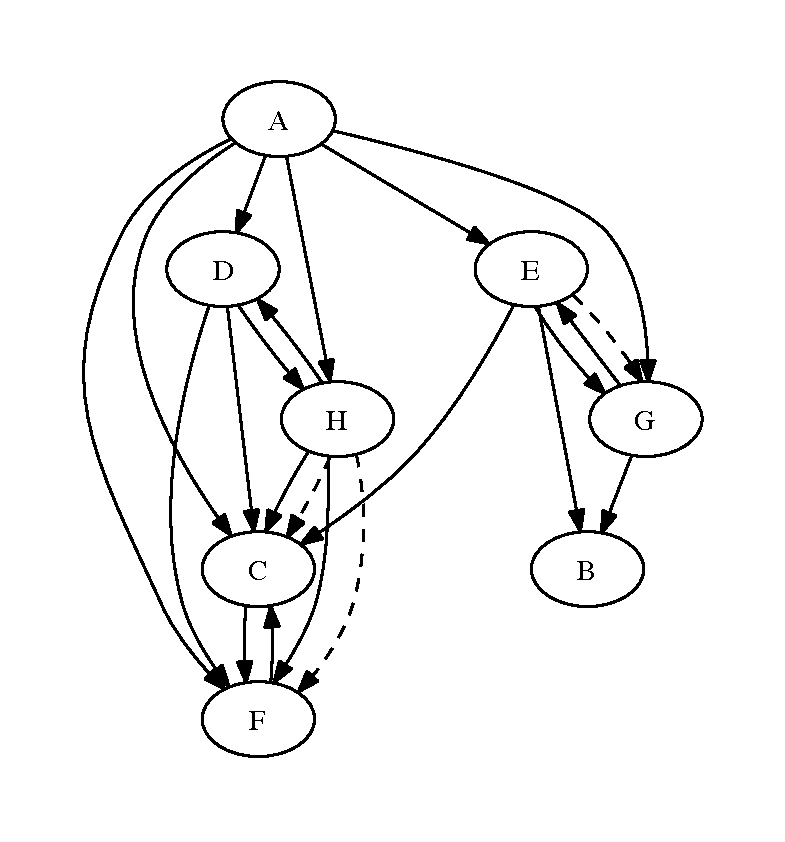
\includegraphics[width=0.5\textwidth]{../SourcesMatlab/electre3-1.pdf}
\caption{Graphe des surclassement sans prise en compte des poids de chaque critère}
\end{center}
\end{figure}

Sur le graphe généré, on voit clairement que la la meilleur solution serait la
solution A car c'est la seule qui n'est dominé par aucune autre.
On voit également que certaines solutions sont équivalentes puisqu'elles se
dominent entres elles. Les couples de solutions \{D, H\}, \{E, G\} et \{C, F\}
sont des couples de solutions équivalentes.
Les solutions F, C et B sont dominés, elles sont donc les moins intéressantes.

Hormis la solution A qui se démarque, il sera difficile d'établir un classement très juste car beaucoup de solutions sont équivalentes entre elles.

\subsection{Avec pondération}

Les pondérations apportés par la partie 2 sont :
\begin{itemize}
\item[g1] : 1.2
\item[g2] : 1.2
\item[g3] : 0.8
\item[g4] : 0.8
\end{itemize}

\clearpage
	
\begin{figure}[!h]
\begin{center}
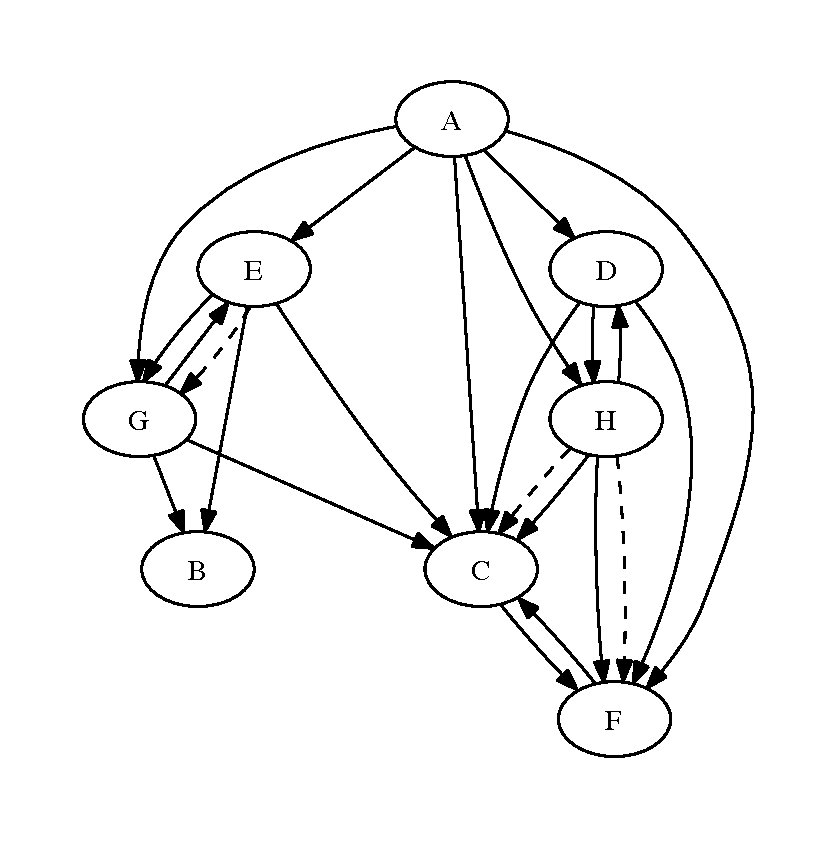
\includegraphics[width=0.5\textwidth]{../SourcesMatlab/electre3-2.pdf}
\caption{Graphe des surclassement avec prise en compte des poids de chaque critère}
\end{center}
\end{figure}

On retrouve la solution A en tête, comme précédemment, et on voit que les positions n'ont pas changé, les surclassement sont presque identiques, seul un surclassement de G sur C est apparu.

\section{Conclusion}

La méthode d'Électre \Rmnum{3} permet de classer un grand nombre de solution suivant plusieurs critères de manière fiable. En pratique elle permet effectivement de tirer des groupes de solutions optimaux d'un ensemble vaste.
Nous avons en effet réussi à isoler une solution optimale parmis les 8 proposés, mais il à été plus difficile d'établir un classement entre toutes les solutions.